\documentclass{beamer}
 
\usepackage[utf8]{inputenc}
\usepackage{graphicx} 
\graphicspath{{img/}}

\usetheme{Copenhagen} 
\title{Containers in a nutshell}
\author{Simone Lombardi}
\institute[HCSSLUG]{
    \textbf{HCSSLUG} \textit{hcsslug.org}
    \newline
    \textit{https://smlb.github.io}
}
\date{27 Ottobre 2017}
\logo{
\includegraphics[height=0.5cm]{hcsslug.png}}  
\begin{document}
 
\frame{\titlepage}

% --------------------------------

\begin{frame}
    \frametitle{Cosa sono i container?}
        I container sono un environment di esecuzione completo ed isolato: hanno a disposizione le loro risorse 
        e condividono con il sistema host il kernel.
\end{frame}

% --------------------------------
     
\begin{frame}
    \frametitle{Vantaggi dei container}
    I container portano numerosi vantaggi: 
    \begin{itemize}
        \item<1-> Portabilit\`a
        \item<2-> Sharing 
        \item<3-> Velocit\`a di deploy 
        \item<4-> Footprint
        \item<5-> Manutenibili
    \end{itemize}
\end{frame}

% --------------------------------

\begin{frame}
    \frametitle{Qualche nome...}
    I progetti pi\`u famosi sono: 
    \begin{itemize}
        \item<1-> LXC
        \item<2-> LXD
        \item<3-> systemd-nspawn 
        \item<4-> Docker 
    \end{itemize}
\end{frame}

% --------------------------------

\begin{frame}
    \frametitle{Docker in a nutshell}
    \begin{center}    
        \includegraphics{{docker_logo.png}}
    \end{center}
\end{frame}

% --------------------------------

\begin{frame}
    \frametitle{Docker in a nutshell}
    Docker \`e un progetto FOSS che estende i Linux container permettendo di buildare e deployare applicativi, usando solo le dipendenze runtime. 
    Mette a disposizione molti tool per gestire i container.
\end{frame}

% --------------------------------

\begin{frame}
    \frametitle{Come funziona Docker?} 
    \begin{itemize}
        \item<1-> \textbf{cgroups}
        \item<2-> \textbf{namespaces}
        \item<3-> \textbf{OverlayFS}
        \item<4-> \textbf{libcontainer}
        \item<5-> \textbf{SELinux}
    \end{itemize}
\end{frame}

% --------------------------------

\begin{frame}
    \frametitle{Perch\`e Docker?}
    \begin{itemize}
        \item<1-> Isolamento degli applicativi
        \item<2-> Creazione e distruzione dei container molto rapida. 
        \item<3-> Velocit\`a e leggerezza
        \item<4-> Risorse condivise col sistema Host
    \end{itemize}
\end{frame}

% ---------------------------------

\begin{frame}
    \frametitle{Un piccolo assaggio}
    Docker pu\`o buildare immagini leggendo un set di istruzioni da un file, chiamato \textbf{Dockerfile}.
    In questo file possiamo definire il comportamento del container e quello che verr\`a eseguito.
    
\end{frame}

% --------------------------------

\begin{frame}
    \frametitle{Dockerfile}
    \begin{center}
        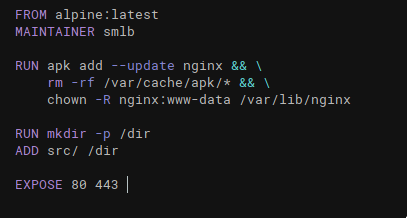
\includegraphics[width=10cm,height=10cm,keepaspectratio]{dockerfile.png}
        \\ \textbf{In figura:} Esempio di Dockerfile
    \end{center}
\end{frame}

% ---------------------------------

\begin{frame}
    \frametitle{Docker: output}
    \begin{center}
        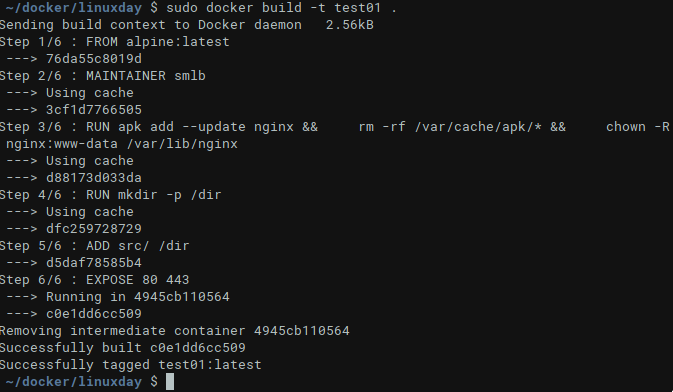
\includegraphics[width=10cm,height=10cm,keepaspectratio]{docker_output.png}
        \\ \textbf{In figura:} Esempio di output 
    \end{center}
\end{frame}

% ---------------------------------

\begin{frame}
    \frametitle{Dockerfile: spiegazione}
    \begin{itemize}
        \item<1->\textbf{FROM}: l'img da cui il tuo container eredita il FS. 
        \item<2->\textbf{RUN}: le direttive di esecuzione per il Dockerfile.
        \item<3->\textbf{ADD}: copia i file dalla source dell'host al path specificato nel container.
        \item<4->\textbf{EXPOSE}: specifica la porta su cui verranno esposti i servizi dal container.
    \end{itemize}
\end{frame}

% --------------------------------

\begin{frame}    
    \frametitle{Altre istruzioni}
    \begin{itemize}
        \item<1-> \textbf{CMD}: a differenza di \textbf{RUN}, non \`e eseguito durante la build ma quando il container \`e inizializzato con l'immagine buildata.
        \item<2-> \textbf{ENV}: usato per settare le variabili di ambiente. 
        \item<3-> \textbf{WORKDIR}: definisce dove \textbf{CMD} sar\`a eseguito. 
        \item<4-> \textbf{ENTRYPOINT} 
    \end{itemize}
\end{frame}

% --------------------------------

\begin{frame}
    \frametitle{Container multipli}
    Vi sono a disposizione innumerevoli tool per gestire applicativi multi-container contemporaneamente, \`e qui che entra in gioco \textbf{Docker Compose}.
\end{frame}

% --------------------------------

\begin{frame}
    \frametitle{Docker Compose}
    \`E un tool per definire e avviare pi\`u container, definiti in un file .yaml, con molte features interessanti:
    \begin{itemize}
        \item<1-> Environments isolati su un singolo host
        \item<2-> I dati dei volumi sono preservati
        \item<3-> \`E possibile ricreare solo i container modificati
    \end{itemize}
\end{frame}

% --------------------------------

\begin{frame}
    \frametitle{Docker Hub}
    \`E un piattaforma che permette di creare repository, buildare immagini e testarle, linkandole a Docker Cloud in modo da permettere 
    il deploy rapido di container.
    \newline
    \begin{center}
        https://hub.docker.com
    \end{center}
\end{frame}

% --------------------------------

\begin{frame}
    \frametitle{Svantaggi di Docker}
    \begin{center}
        \textbf{Confronto con le VM}
    \end{center}
    \begin{itemize}
        \item<1-> Le VM possono essere `spostate` mentre sono in esecuzione. 
        \item<2-> I Container \textbf{NON} rimpiazzano le VM in ogni caso.
        \item<3-> Valutare sempre gli USE Case!
    \end{itemize}
\end{frame}

% --------------------------------

\begin{frame}
    \frametitle{VM vs Docker: layers}
    \begin{center}
        \includegraphics[width=9cm,height=9cm,keepaspectratio]{{vmvsdocker.png}}
    \end{center}
\end{frame}

% --------------------------------

\begin{frame}
    \frametitle{Conclusione}
    Docker \`e uno strumento molto versatile, permette di gestire workflow e infrastrutture in maniera pulita e davvero intuitiva. Le casistiche di utilizzo
    sono molteplici, come per ogni tipo di strumento, bisogna sempre valutarne i pro e i contro.
\end{frame}

% --------------------------------

\begin{frame}
    \frametitle{Fine}
    \begin{center}
        \~{} \#{} docker stop linuxday 
        \newline
        \newline
        \textbf{Grazie a tutti per l'attenzione :D}
    \end{center}
\end{frame}

% --------------------------------

\end{document}
